\documentclass[11pt,a4paper]{article}

\usepackage[margin=2cm]{geometry}
\usepackage{amsmath}
\usepackage{amssymb}
\usepackage{xcolor}
\usepackage{tikz}
\usepackage{pgfplots}
\pgfplotsset{compat=1.18}
\usepackage[most]{tcolorbox}
\usepackage{enumitem}
\setlist[itemize]{leftmargin=1.4em, itemsep=2pt, topsep=2pt}

% --- colours ---
\definecolor{ch1col}{HTML}{1F6FB2}   % CH1 / supply
\definecolor{ch2col}{HTML}{C0392B}   % CH2 / V_LED
\definecolor{barcol}{HTML}{2E7D5B}
\definecolor{notefill}{HTML}{F1F5FA}
\definecolor{noteline}{HTML}{1F6FB2}

\pgfplotsset{
  scopestyle/.style={
    width=12cm, height=5.2cm, grid=both,
    grid style={gray!18}, axis line style={gray!55},
    tick label style={font=\footnotesize}, label style={font=\small},
    enlarge x limits=false
  }
}

\newtcolorbox{notebox}[1]{
  colback=notefill, colframe=noteline, boxrule=0.5pt,
  left=8pt,right=8pt,top=6pt,bottom=6pt,
  fonttitle=\bfseries, title=#1, coltitle=white, colbacktitle=noteline
}

\setlength{\parindent}{0pt}
\setlength{\parskip}{4pt}

\begin{document}

\begin{center}
{\LARGE\bfseries Day 2 --- Lab Record}\\[2pt]
{\large Expected instrument readings \& key notes}\\[4pt]
{\small First circuit, variable resistance, voltage dividers \quad(no screenshots were taken --- these are the expected views)}
\end{center}

\hrule
\vspace{6pt}

\textbf{Which instrument each lab used:}
\begin{itemize}
  \item \textbf{Lab 1 (KVL)} and \textbf{Lab 4 (pot $\to$ LED)} were observed on the \textbf{oscilloscope} --- so each has an expected \emph{scope trace} below.
  \item \textbf{Lab 2 (Ohm's law sweep)} and \textbf{Lab 3 (divider loading)} were measured with the \textbf{DMM} --- a voltage scope would not show current directly, and the DC voltages would simply appear as flat lines, so these are shown as the graph the readings actually produce.
\end{itemize}

% ===================== LAB 1 =====================
\section*{Lab 1 --- KVL on 9\,V $+$ 470\,$\Omega$ $+$ red LED \hfill\normalfont\small (scope, DC coupled)}

Nodes: \textbf{A} = supply ($+$), \textbf{B} = junction between 470\,$\Omega$ and LED, \textbf{C} = LED cathode $=$ supply $-$ $=$ ground.
\textbf{Both probe ground clips at C.} CH1 tip at A, CH2 tip at B.

\begin{center}
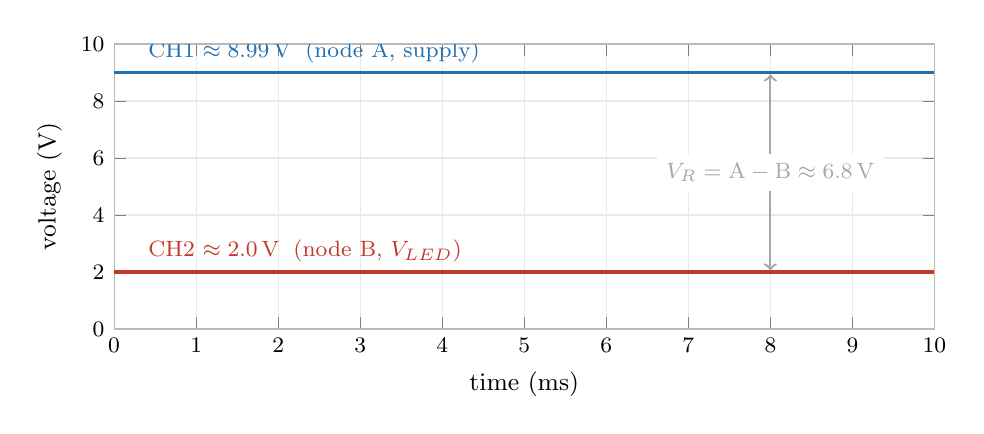
\begin{tikzpicture}
\begin{axis}[scopestyle, xlabel={time (ms)}, ylabel={voltage (V)},
  xmin=0, xmax=10, ymin=0, ymax=10, ytick={0,2,4,6,8,10}]
  \addplot[ch1col, very thick, domain=0:10, samples=2]{8.99};
  \addplot[ch2col, very thick, domain=0:10, samples=2]{2.0};
  \node[ch1col, anchor=south west, font=\footnotesize] at (axis cs:0.3,8.99){CH1 $\approx 8.99$\,V \;(node A, supply)};
  \node[ch2col, anchor=south west, font=\footnotesize] at (axis cs:0.3,2.0){CH2 $\approx 2.0$\,V \;(node B, $V_{LED}$)};
  \draw[<->, thick, gray!70] (axis cs:8,2.05) -- (axis cs:8,8.94)
        node[midway, fill=white, font=\footnotesize]{$V_R = \mathrm{A}-\mathrm{B}\approx 6.8$\,V};
\end{axis}
\end{tikzpicture}
\end{center}

\begin{itemize}
  \item A DC circuit shows as \textbf{flat horizontal lines} on the scope --- nothing varies with time.
  \item The scope's value here is reading \textbf{two nodes at once}; the \textbf{Math channel ($\mathrm{A}-\mathrm{B}$)} gives $V_R$ directly.
  \item \textbf{KVL check:} $V_R + V_{LED} = 6.8 + 2.0 = 8.8\,$V $\approx$ the measured supply $8.99\,$V. \checkmark
\end{itemize}

% ===================== LAB 2 =====================
\section*{Lab 2 --- Ohm's law from a current sweep \hfill\normalfont\small (DMM in series, LED removed)}

Just a resistor across the $\approx 9$\,V supply; DMM in \textbf{mA} mode, \textbf{in series}, so all current is read. $I = V/R$.

\begin{center}
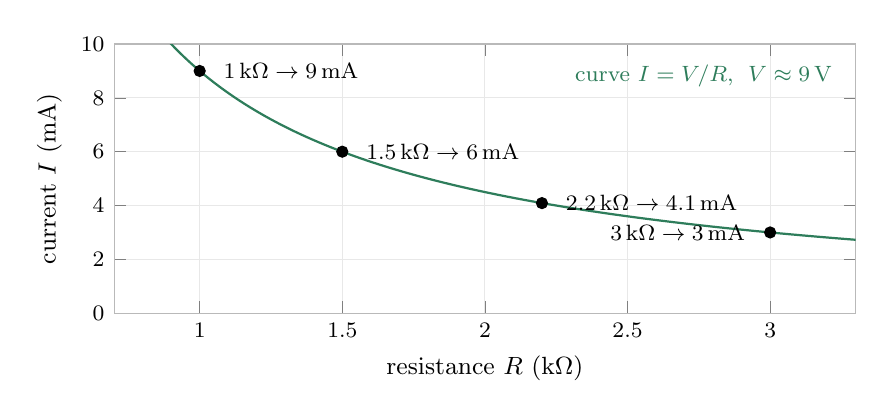
\begin{tikzpicture}
\begin{axis}[width=11cm, height=5cm, grid=both, grid style={gray!18},
  axis line style={gray!55}, tick label style={font=\footnotesize}, label style={font=\small},
  xlabel={resistance $R$ (k$\Omega$)}, ylabel={current $I$ (mA)},
  xmin=0.7, xmax=3.3, ymin=0, ymax=10]
  \addplot[barcol, thick, domain=0.7:3.3, samples=120]{9/x};
  \addplot[only marks, mark=*, mark size=2pt, black] coordinates {(1,9)(1.5,6)(2.2,4.09)(3,3)};
  \node[anchor=west, font=\footnotesize] at (axis cs:1.05,9){$1\,$k$\Omega\to 9\,$mA};
  \node[anchor=west, font=\footnotesize] at (axis cs:1.55,6){$1.5\,$k$\Omega\to 6\,$mA};
  \node[anchor=west, font=\footnotesize] at (axis cs:2.25,4.09){$2.2\,$k$\Omega\to 4.1\,$mA};
  \node[anchor=west, font=\footnotesize] at (axis cs:3.0,3){\hspace{-2.4cm}$3\,$k$\Omega\to 3\,$mA};
  \node[barcol, anchor=north east, font=\footnotesize] at (axis cs:3.25,9.6){curve $I=V/R$, \;$V\approx 9$\,V};
\end{axis}
\end{tikzpicture}
\end{center}

\begin{itemize}
  \item Points sit on the $I = V/R$ curve, so \textbf{$V = I\cdot R \approx 9$\,V} at every value --- that constancy \emph{is} Ohm's law confirmed.
  \item Halving doesn't apply here, but note current \textbf{rises as $R$ falls} (a brighter-LED intuition from earlier).
\end{itemize}

% ===================== LAB 3 =====================
\section*{Lab 3 --- Divider loading \hfill\normalfont\small (DMM at the mid-point)}

$10\,$k top, $10\,$k bottom, $5$\,V supply. Unloaded mid-point $=2.50$\,V, so $V_{Th}=2.5$\,V and $R_{Th}=10\text{k}\,\|\,10\text{k}=5\,$k$\Omega$.
Each load forms a divider with $R_{Th}$: $\;V = V_{Th}\dfrac{R_L}{R_{Th}+R_L}$.

\begin{center}
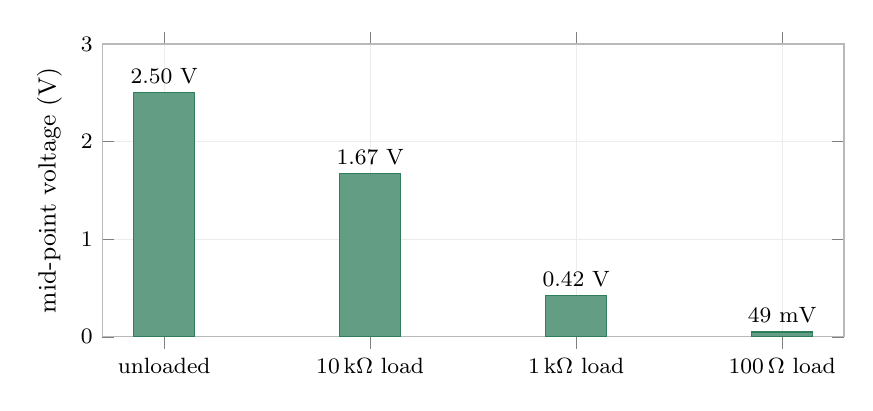
\begin{tikzpicture}
\begin{axis}[ybar, width=11cm, height=5.3cm, bar width=22pt,
  ymin=0, ymax=3, ylabel={mid-point voltage (V)},
  symbolic x coords={unloaded,L10k,L1k,L100},
  xticklabels={unloaded,$10\,$k$\Omega$ load,$1\,$k$\Omega$ load,$100\,\Omega$ load},
  xtick=data, tick label style={font=\footnotesize}, label style={font=\small},
  nodes near coords, point meta=explicit symbolic,
  every node near coord/.append style={font=\footnotesize},
  grid=both, grid style={gray!15}, axis line style={gray!55}]
  \addplot[fill=barcol!75, draw=barcol] coordinates {
     (unloaded,2.50) [2.50 V]
     (L10k,1.67)     [1.67 V]
     (L1k,0.42)      [0.42 V]
     (L100,0.049)    [49 mV]
  };
\end{axis}
\end{tikzpicture}
\end{center}

\begin{itemize}
  \item The output is \textbf{not} a stiff $2.5$\,V --- it \textbf{drops} as the load shrinks. This is the Thévenin story made visible.
  \item Smaller load $\Rightarrow$ more current through $R_{Th}$ $\Rightarrow$ bigger drop across it. (Full working is in the EOD write-up.)
  \item On a scope each of these would simply be a \textbf{flat DC line} at that voltage.
\end{itemize}

% ===================== LAB 4 =====================
\section*{Lab 4 --- Pot-controlled LED \hfill\normalfont\small (scope on the wiper, DC coupled)}

$10$\,k pot ends to $5$\,V / GND; wiper $\to 470\,\Omega \to$ LED $\to$ GND. Turning the pot sweeps the wiper voltage; the curve below is wiper voltage vs rotation. On the scope this appears as a \textbf{flat line at the wiper voltage} that slides up or down as you turn.

\begin{center}
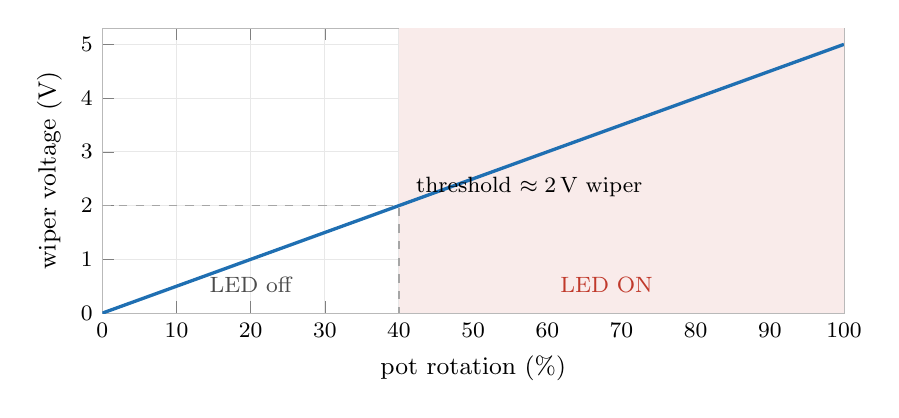
\begin{tikzpicture}
\begin{axis}[scopestyle, width=11cm, xlabel={pot rotation (\%)}, ylabel={wiper voltage (V)},
  xmin=0, xmax=100, ymin=0, ymax=5.3, ytick={0,1,2,3,4,5}]
  \fill[ch2col!10] (axis cs:40,0) rectangle (axis cs:100,5.3);
  \addplot[ch1col, very thick, domain=0:100, samples=2]{5*x/100};
  \draw[dashed, gray!70] (axis cs:0,2)--(axis cs:40,2)--(axis cs:40,0);
  \node[anchor=south, font=\footnotesize, ch2col] at (axis cs:68,0.2){LED ON};
  \node[anchor=south, font=\footnotesize, gray!60!black] at (axis cs:20,0.2){LED off};
  \node[anchor=west, font=\footnotesize] at (axis cs:41,2.35){threshold $\approx 2$\,V wiper};
\end{axis}
\end{tikzpicture}
\end{center}

\begin{itemize}
  \item Below $\sim 2$\,V at the wiper the LED is \textbf{off} (its $\approx 2$\,V forward drop isn't met); above it, brightness rises with wiper voltage.
  \item The $470\,\Omega$ sets the current: $I=(V_{wiper}-2)/470$, reaching $\approx 6.4$\,mA at a $5$\,V wiper.
\end{itemize}

\vspace{4pt}
% ===================== NOTES =====================
\begin{notebox}{Key conceptual notes (worth keeping)}
\begin{itemize}
  \item \textbf{LED:} clamps its forward voltage at $\approx 2$\,V but does \emph{not} limit current; \textbf{current (heat) is what destroys it}, so the series resistor's real job is to \textbf{limit current} --- $I=(V-2)/470$. You can't use $V/(R+R_{LED})$ because the LED is nonlinear; subtract the $\approx 2$\,V and use the resistor.
  \item \textbf{Potentiometer:} one resistive track \emph{split by the wiper} into $R_{top}+R_{bot}$ (always summing to $10$\,k). The wiper is a \textbf{node, not a component}; its voltage is the divider output. The $470\,\Omega+$LED is a \textbf{separate branch} hanging off the wiper node.
  \item \textbf{Parallel vs series (the key one):} parallel branches \textbf{always share the same voltage}; any voltage \textbf{``drop''/droop is a \emph{series} effect} across $R_{top}$. With $R_{top}=0$ there is no series resistance to drop voltage, so the wiper sits at the \textbf{full 5\,V} and both parallel branches see $5$\,V at different currents.
  \item \textbf{Scope grounding:} all probe ground clips are internally \textbf{common and earth-tied} $\Rightarrow$ \textbf{tie every ground clip to one circuit-ground node}, or two clips will short two points together (this had shorted the LED earlier).
  \item \textbf{Th\'evenin / loading:} any linear two-terminal network looks like $V_{Th}$ in series with $R_{Th}$; a load forms a divider with $R_{Th}$, so the output droops. (Recipe and worked example in the EOD write-up.)
\end{itemize}
\end{notebox}

\end{document}
